%   Filename    : chapter_4.tex 
\chapter{Preliminary Results/System Prototype}
This chapter presents the preliminary results of the study, including findings from data gathering, the system's diagrams and designs, initial user interface (UI) for the front end, and the chatbot's architecture.

\section{Data Gathering Results}
The research process for developing TUKIB started with a comprehensive visit to the UPV RRC during the researchers' internship. This phase involved engaging with key personnel and understanding the intricacies of the center's operations. The following sections detail the key activities and information undertaken and gathered during this visit.

\subsection{Facility Tour}
During the researcher's visit, they met with the center's director, administrative staff, and laboratory heads. This introduction provided valuable insights into the roles and responsibilities of various individuals and departments within the RRC. Understanding these dynamics was crucial for tailoring the system to fit the center’s workflows.

The researchers were also given a guided tour, which provided an overview of various laboratories and services offered. These services includes:

\begin{itemize}
	\item \textbf{Sample Processing.}The RRC provides critical sample processing services, essential for research and analysis.
	\item \textbf{Laboratory Equipment Rental} Various pieces of laboratory equipment are available for rent, which supports a wide range of scientific projects.
	\item \textbf{Training and Workshops.} The RRC offers training sessions on laboratory equipment, promoting user proficiency.
	\item \textbf{Facility Rentals.} Access to spaces like the Audio-Visual Room (AVR) and conference rooms was noted as a valuable resource for users.
\end{itemize}

Each laboratory, including the Biology, Microbiology, Nanotechnology, and Applied Chemistry labs, was introduced in detail, with specific equipment and services discussed in terms of their availability and purpose. The UPV RRC houses five (5) laboratories, namely: Biology, Microbiology, Nanotechnology, Applied Chemistry Laboratory, and Food, Feeds, and Functional Nutrition Laboratory.

\subsection{Stakeholder identification and engagement}
The success of workflow automation hinges on understanding the needs and expectations of its key stakeholders. These stakeholders include the RRC laboratory and administrative staff, the clients (university and student researchers and external users of the RRC facilities), the developers, and the member/s of the Computer Science Faculty guiding the project.

The researcher's interaction with the stakeholders allowed them to gather valuable feedback on the existing system and the challenges they faced. This feedback played a crucial role in shaping the direction of our system design, as it highlighted the need for automation, service tracking, and streamlined communication between stakeholders. This in-depth exposure to the center’s operations was essential for the initial design and development phase of TUKIB, providing a strong foundation for creating a system tailored to the specific needs of the RRC and other research institutions with similar setups.

\subsection{Scope and Limitations of the Services}
Through direct discussions with the center’s director and administrative staff, the researchers obtained a clear picture of the scope of services provided by each facility, as well as the current limitations they face. Some of these limitations included:

\begin{itemize}
	\item The UPV RRC currently has no website describing its mission, vision, services offered, service request steps, or other relevant information. This limits clients from acquiring relevant knowledge on how the center's service operates.
	\item Access to certain equipment is restricted due to varying availability, as it is essential to ensure that no one else is using it before it can be rented out.
	\item A manual service request and data management system reliant on Google Forms and Sheets, which posed challenges in efficiency and scalability.
\end{itemize}

\section{System Design}

\subsection{Context Model}

\begin{figure}[h]
	\centering 
	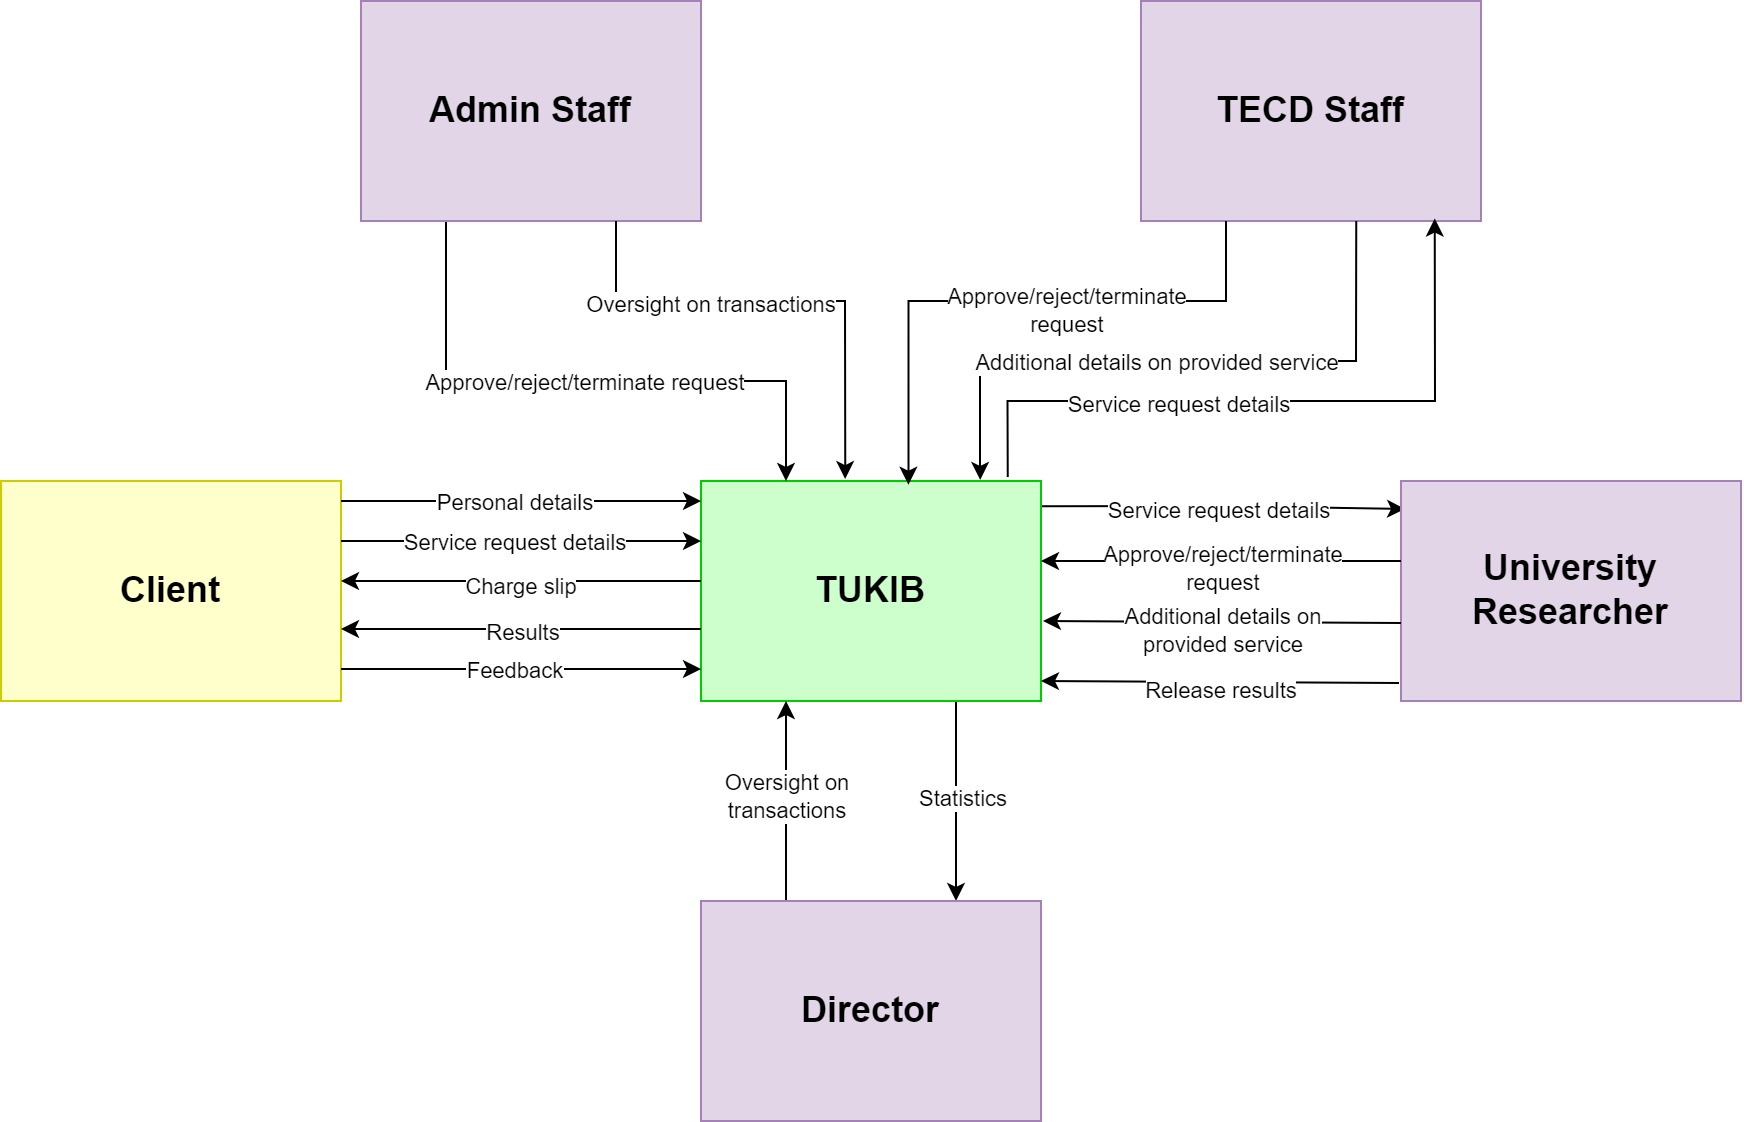
\includegraphics[width=1\textwidth]{context model.png}
	\caption{Context model for the interactions of internal and external entities with TUKIB}
	\label{fig:context_model}
\end{figure}

\subsection{Process Flow Diagram}

\subsection{Data Flow Diagram}

\subsection{Database Diagram}

\subsection{Chatbot Conversation Flow}

\section{User Interface}

\subsection{Landing Page}

\subsection{User Authentication}